\subsection{Open Loop Control}
	The DoodleBot uses two stepper motors in an open loop arrangement to control the position and movement of the drawing head. The input to the system is the frequency of voltage pulses and the output is the dynamics of the drawing head. For this system to operate properly, there are constraints on the maximum acceleration the system can run at.
	
	Both the input and output operate in 'step' units (see Section~\ref*{sec:implementation-mechanical} for more detail on what this unit is in the real system).
	
\subsection{Stepper Motors and Open Loop Justification}
		\label{sec:control-stepper}
			
		Stepper Motors are brushless DC motors used as the primary drivers for X and Y movement in the DoodleBot. 
		
		Where a standard DC motor produces an output torque proportional to input current, a stepper motor rotates at an output speed equal to the input frequency of received voltage pulses. Fundamentally, they are very different devices.
		
		\begin{figure}[h]
			\centering
			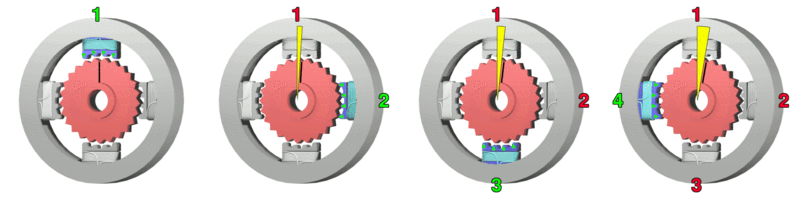
\includegraphics[width=0.8\textwidth]{figures/optimisation/steppermotor}
			\caption[Operation of a simple stepper motor]{Operation of a simplified stepper motor over four steps. \textit{Source: Wapcaplet; Trevolt. Gif of Wapcaplet's 
			4 images. Wikimedia Commons.\cite{website:stepper}}}
			\label{fig:stepper}
		\end{figure}
		
		As shown in Figure~\ref{fig:stepper}, stepper motors consist of several electromagnets arranged in a equally spaced pattern around a gear-shaped rotor. Each electromagnet has 'teeth' that can align with the rotor's 'teeth'. The activation of the electromagnets are controlled by a stepper motor driver, which is considered to be part of the stepper motor component for the modelling of the system.
		
		When the stepper motor driver receives a single voltage step input, it provides a constant current to the first electromagnet, creating magnetic force that rotates the rotor a small amount (a single step) such that the teeth on the rotor gear align with the teeth on the magnet. Damping in the mechanical system prevent oscillations about this point and as long as the input voltage pulse is maintained, this electromagnet will remain active.
		
		When the first electromagnet is aligned with the rotor teeth, the second electromagnet will be out of alignment. When a second input voltage pulse is received by the stepper motor driver, the second electromagnet is activated, causing the rotor to make another rotation step such that it is now in alignment with the second electromagnet. This process continues sequentially across numerous electromagnets around the rotor.
		
		The important thing to note is that the speed of rotation is proportional to the frequency in which the input voltage pulses are received and is not effected by varying mechanical load. As long as the magnetic force provided by the electromagnet is enough for the rotor to make the required step within the time the electromagnet is active, the average speed will always remain the same. A lighter load may allow the individual step to be quicker, but as the second step will not be made until the next input pulse is received, the differences between a heavy and light load are not noticeable.
		
		If however, the load is large enough such that the magnetic force is not enough to make the required step within the activation time of the electromagnet, then the stepper motor will be in the wrong state for the next motion (the teeth of the rotor will be in the wrong position relative to the second electromagnet). The whole system goes out of phase and stops moving in a predictable fashion (in fact, speed drops significantly and the motor barely turns, despite input pulses being received). So when this threshold is reached, the motors can be considered to be completely inoperable.
		
		So this means that within certain torque constraints, the stepper motor is a robust and predictable device that can be run in open loop. Since the loads on the system do not vary significantly between possible states (the gravitational force is always the same orientation for all states and mass is constant) the torque constraints can be approximated by an acceleration constraints making the model of the system a lot simpler and easier to design for.